\documentclass{article}
\usepackage{amsmath}
\usepackage{amsfonts}
\usepackage{amssymb}
\usepackage{fancyref}
\usepackage{amsmath}
\usepackage{tikz}
\usepackage{listings}
\usepackage{xcolor}
\usetikzlibrary{arrows.meta, positioning}

\title{LSTM Formulas - PyTorch Implementation}
\author{Tobias}
\date{\today}

% Define Python style for highlighting
\lstdefinestyle{python}{
    language=Python,
    basicstyle=\ttfamily\small,
    keywordstyle=\bfseries\color{blue},
    stringstyle=\color{green},
    commentstyle=\color{gray},
    showstringspaces=false,
    frame=single,
    breaklines=true
}

\begin{document}

\maketitle

\section{Introduction}
The Long Short-Term Memory (LSTM) is a type of recurrent neural network (RNN) designed to model sequences and dependencies over time. Below are the key equations that define the LSTM, following the PyTorch-style implementation.

\section{LSTM Equations}

\subsection{Input Gate}
The input gate decides which values to update in the cell state. In the PyTorch-style implementation, the input gate is computed as:
\begin{equation}
i_t = \sigma(W_{ii} x_t + b_{ii} + W_{hi} h_{t-1} + b_{hi})
\label{eq:input_gate}
\end{equation}

\subsection{Forget Gate}
The forget gate determines which parts of the previous cell state to keep:
\begin{equation}
f_t = \sigma(W_{if} x_t + b_{if} + W_{hf} h_{t-1} + b_{hf})
\end{equation}

\subsection{Cell State Update}
The candidate cell state is computed as:
\begin{equation}
\tilde{C}_t = \tanh(W_{ig} x_t + b_{ig} + W_{hg} h_{t-1} + b_{hg})
\end{equation}
The new cell state is updated using the forget and input gates:
\begin{equation}
C_t = f_t \odot C_{t-1} + i_t \odot \tilde{C}_t
\end{equation}

\subsection{Output Gate}
The output gate controls the hidden state and final output:
\begin{equation}
o_t = \sigma(W_{io} x_t + b_{io} + W_{ho} h_{t-1})
\end{equation}
The hidden state is then updated as:
\begin{equation}
h_t = o_t \odot \tanh(C_t)
\end{equation}

\section{Notation}
\begin{itemize}
    \item $x_t$: Input at time step $t$
    \item $h_{t-1}$: Hidden state from the previous time step
    \item $C_t$: Cell state at time step $t$
    \item $W_{ii}, W_{if}, W_{ig}, W_{io}$: Weight matrices for the input applied to input, forget, candidate cell, and output gates
    \item $W_{hi}, W_{hf}, W_{hg}, W_{ho}$: Weight matrices for the hidden state applied to input, forget, candidate cell, and output gates
    \item $b_{ii}, b_{if}, b_{ig}, b_{io}$: Biases for input, forget, candidate cell, and output gates
    \item $\sigma$: Sigmoid activation function
    \item $\tanh$: Hyperbolic tangent activation function
    \item $\odot$: Element-wise multiplication (Hadamard product)
\end{itemize}

\subsection{LSTM Inputs and Outputs}
At each time step \( t \), the Long Short-Term Memory (LSTM) unit takes the current input \( x_t \) and the previous hidden state \( h_{t-1} \) as inputs. It also utilizes the previous cell state \( C_{t-1} \) to compute two key outputs: the hidden state \( h_t \) and the cell state \( C_t \). The hidden state \( h_t \) represents the output of the LSTM at time step \( t \) and is often used for tasks such as sequence prediction. The cell state \( C_t \) carries information across time steps, managing long-range dependencies. While both \( h_t \) and \( C_t \) are produced at each time step, the primary output used in further computations is typically the hidden state \( h_t \).

\subsection{Relevance propagation}
\subsubsection{Basics}
First we'll take a step back and look at the basic building blocks of the LSTM and calculate the relevance propagation for each component. The relevance propagation is a technique used to understand the contribution of each input to the output of a neural network. By calculating the relevance propagation, we can identify which parts of the input are most relevant to the output, providing insights into the model's decision-making process.

\section{Linear Layer with Tanh Activation}

Consider a linear layer with 3 inputs and 1 output. The inputs and weights are defined as follows:
\[
\begin{aligned}
x_1 &= 0.1, \quad w_1 = 1 \\
x_2 &= 0.2, \quad w_2 = 2 \\
x_3 &= 0.3, \quad w_3 = 3
\end{aligned}
\]

The output \( y \) of the linear layer can be calculated as:
\[
y = w_1 x_1 + w_2 x_2 + w_3 x_3 = 1 \cdot 0.1 + 2 \cdot 0.2 + 3 \cdot 0.3 = 1.4
\]

Next, we apply the hyperbolic tangent activation function:
\[
\text{output} = \tanh(y) = \tanh(1.4) \approx 0.8854
\]

\section{Network Visualization}

\begin{center}
    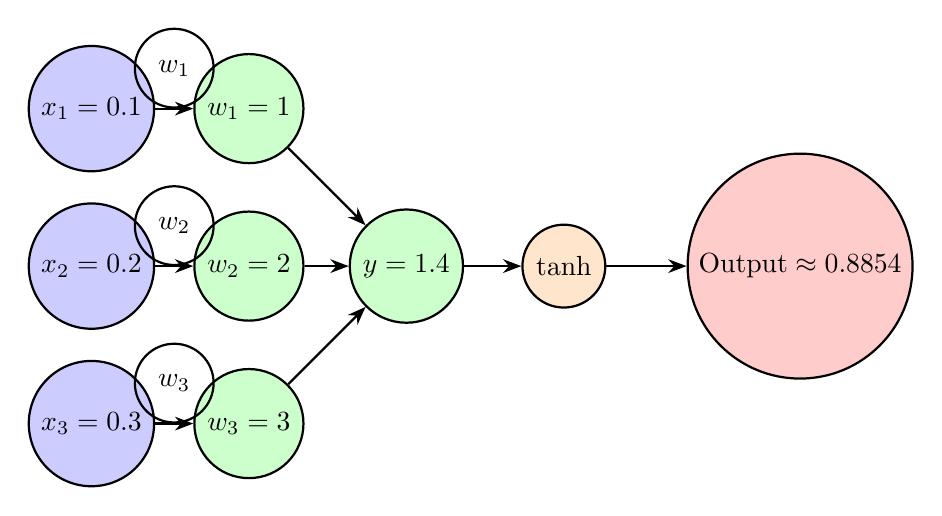
\begin{tikzpicture}[
        every node/.style={draw, circle, minimum size=1cm},
        input/.style={fill=blue!20},
        output/.style={fill=red!20},
        tanh/.style={fill=orange!20},
        neuron/.style={fill=green!20},
        thick,
        ->,
        >=Stealth
    ]
    
    % Input Nodes
    \node[input] (x1) at (0, 2) {$x_1 = 0.1$};
    \node[input] (x2) at (0, 0) {$x_2 = 0.2$};
    \node[input] (x3) at (0, -2) {$x_3 = 0.3$};
    
    % Weight Nodes
    \node[neuron] (w1) at (2, 2) {$w_1 = 1$};
    \node[neuron] (w2) at (2, 0) {$w_2 = 2$};
    \node[neuron] (w3) at (2, -2) {$w_3 = 3$};
    
    % Linear Layer Output
    \node[neuron] (linear) at (4, 0) {$y = 1.4$};
    
    % Tanh Activation Node
    \node[tanh] (tanh) at (6, 0) {tanh};
    
    % Tanh Activation Output
    \node[output] (output) at (9, 0) {$\text{Output} \approx 0.8854$};
    
    % Draw Arrows with Weights
    \draw[->] (x1) edge node[above] {$w_1$} (w1);
    \draw[->] (x2) edge node[above] {$w_2$} (w2);
    \draw[->] (x3) edge node[above] {$w_3$} (w3);
    \draw[->] (w1) -- (linear);
    \draw[->] (w2) -- (linear);
    \draw[->] (w3) -- (linear);
    \draw[->] (linear) -- (tanh);
    \draw[->] (tanh) -- (output);
    
    \end{tikzpicture}
    \end{center}
The layer-wise values for this are as follows:
\begin{equation}
\begin{aligned}
    R\left[x_{1}\right] = \frac{\tanh(1.4)}{1.4} \cdot 1 \cdot 0.1 = 0.063 \\
    R\left[x_{2}\right] = \frac{\tanh(1.4)}{1.4} \cdot 2 \cdot 0.2 = 0.253 \\
    R\left[x_{3}\right] = \frac{\tanh(1.4)}{1.4} \cdot 3 \cdot 0.3 = 0.569
\end{aligned}
\end{equation}

Till here, DeepLift and LRP are the same. However, the difference arises when there is a bias involved.
Then in case of DeepLift the relevance is calculated as:

\begin{equation}
r[x_{i}] = \frac{\tanh(1.4) - \tanh(w_{i} * x_{i, \text{baseline}})}{1.4}w_{i} \cdot x_{i}
\end{equation}

For LRP, without a baseline this results to:
\begin{equation}
r[x_{i}] = \tanh(1.4)\frac{x_{i}w_{i}}{1.4}
\end{equation}

Or to generalize:
\begin{equation}
\textbf{r}[\textbf{x}] = \tanh(\textbf{w}\textbf{x} + \textbf{b})\frac{\textbf{w}\odot\textbf{x}}{\textbf{w}\textbf{x} + \textbf{b}}
\end{equation}
Unfortunately, this does violate the additivity principle (but this is how it's implemented in captum). 
We can conserve this though by not accounting for the bias in the linear layer.
\begin{equation}
\textbf{r}[\textbf{x}] = \tanh(\textbf{w}\textbf{x} + \textbf{b})\frac{\textbf{w}\odot\textbf{x}}{\textbf{w}\textbf{x}}
\end{equation}

Code to follow along:
\begin{lstlisting}[style=python]
    from captum.attr import LRP
    from torch import nn
    import torch
    import torch.nn.functional as F
    from shap import DeepExplainer
    
    class SimpleModel(nn.Module):
        def __init__(self):
            super().__init__()
            self.tanh = nn.Tanh()
            self.fc = nn.Linear(in_features=3, out_features=1)
    
        def forward(self, x):
            x = self.fc(x)
            x = self.tanh(x)
            return x
    
    model = SimpleModel()
    weights = torch.tensor([[1., 2., 3.]], dtype=torch.float32)
    bias = torch.tensor([0.0], dtype=torch.float32)
    model.fc.weight.data = weights
    model.fc.bias.data = bias
    
    lrp = LRP(model)
    
    x = torch.tensor([[0.1, 0.2, 0.3]], dtype=torch.float32)
    attribution = lrp.attribute(x, target=0)
    output = model(x)
    
    # lrp attribution
    manual_attribution = torch.tanh(F.linear(weights, x, bias)) * weights * x / F.linear(weights, x, bias)

    # DeepLift attribution as used by shap
    x_baseline = torch.tensor([[0.0, 0.0, 0.0], [0.,0.,0.]], dtype=torch.float32)
    exp = DeepExplainer(model, x_baseline)
    values = exp(x)

    manual_values = (torch.tanh(F.linear(weights, x, bias)) - torch.tanh(F.linear(weights, torch.Tensor([[0., 0., 0.]]), bias))) / F.linear(weights, x) * weights * x
\end{lstlisting}

For the DeepLift implementation, we can use the following:
\begin{equation}
\textbf{r}[\textbf{x}] = (\tanh(\textbf{w}\textbf{x} + \textbf{b}) - \tanh(\textbf{w}\textbf{x}_{\text{baseline}} + \textbf{b}))\frac{\textbf{w}\odot\textbf{x}}{\textbf{w}\textbf{x}}
\end{equation}


Now how does this translate to matrices $\textbf{W}$?
This works equally for matrices, but we need to account for the contribution of each neuron in the layer (in contrast to just one we had prior) attributing to the relevance scores to the `i`-th output:

\begin{equation}
\textbf{r}[\textbf{x}]_{i} = \tanh(\textbf{W}[i, :]\textbf{x} + \textbf{b})\frac{\textbf{W}[i,:]\odot\textbf{x}}{\textbf{W}[i, :]\textbf{x}}
\end{equation}

\subsubsection{LSTM}
With this we are set to calculate the relevance propagation for the LSTM.

We work our way through the formulas \eqref{eq:input_gate}, (todo: add others) and calculate the relevance propagation for each component.
We start with
\begin{equation}
    \tag{input gate - LRP}
R\left[x_{t}\right] = \sigma(\textbf{W}_{ii} x_t + \textbf{b}_{ii} + \textbf{W}_{hi} \textbf{h}_{t-1})\frac{\textbf{W}_{ii} \odot \textbf{x}_{t}}{\textbf{W}_{ii} \textbf{x}_t + \textbf{b}_{ii} + \textbf{W}_{hi} \textbf{h}_{t-1}}
\end{equation}

\begin{equation}
    \tag{input gate - Adjusted LRP}
\textbf{r}\left[\textbf{x}_{t}\right] = \sigma(\textbf{W}_{ii} x_t + \textbf{b}_{ii} + \textbf{W}_{hi} \textbf{h}_{t-1})\frac{\textbf{W}_{ii} \odot \textbf{x}_{t}}{\textbf{W}_{ii} \textbf{x}_t}
\end{equation}

shap always calculates both: $\textbf{r}\left[\textbf{x}_{t}\right]$ and $\textbf{r}\left[\textbf{h}_{t-1}\right]$.
input gate - DeepLift - Rx
\begin{equation}
\begin{aligned}
\textbf{r}\left[\textbf{x}_{t}\right] = (\sigma(\textbf{W}_{ii} \textbf{x}_t + \textbf{b}_{ii} + \textbf{W}_{hi} \textbf{h}_{t-1}) - \\
\sigma(\textbf{W}_{ii} \textbf{x}_{\text{baseline}} + \textbf{b}_{ii} + \textbf{W}_{hi} \textbf{h}_{\text{baseline}} + \textbf{b}_{hi})) \\
\frac{\textbf{W}_{ii} \odot \textbf{x}_{t}}{\textbf{W}_{ii} \textbf{x}_t + \textbf{W}_{hi} \textbf{h}_{t-1}}
\end{aligned}
\end{equation}


input gate - DeepLift - Rh
\begin{equation}
\begin{aligned}
\textbf{r}\left[\textbf{h}_{t-1}\right] = (\sigma(\textbf{W}_{ii} \textbf{x}_t + \textbf{b}_{ii} + \textbf{W}_{hi} \textbf{h}_{t-1} + \textbf{b}_{hi}) - \\
 \sigma(\textbf{W}_{ii} \textbf{x}_{\text{base}} + \textbf{b}_{ii} + \textbf{W}_{hi} \textbf{h}_{\text{base}} + \textbf{b}_{hi})) \cdot \\
\frac{\textbf{W}_{hi} \odot \textbf{h}_{t-1}}{\textbf{W}_{ii} \textbf{x}_t + \textbf{W}_{hi} \textbf{h}_{t-1}}
\end{aligned}
\end{equation}

Forget Gate (works analogously to Input gate):

forget gate - DeepLift - Rx
\begin{equation}
\begin{aligned}
\textbf{r}\left[\textbf{x}_{t}\right] = (\sigma(\textbf{W}_{if} \textbf{x}_t + \textbf{b}_{if} + \textbf{W}_{hi} \textbf{h}_{t-1}) - \\
\sigma(\textbf{W}_{if} \textbf{x}_{\text{baseline}} + \textbf{b}_{if} + \textbf{W}_{hf} \textbf{h}_{\text{baseline}} + \textbf{b}_{hf})) \\
\frac{\textbf{W}_{if} \odot \textbf{x}_{t}}{\textbf{W}_{if} \textbf{x}_t + \textbf{W}_{hf} \textbf{h}_{t-1}}
\end{aligned}
\end{equation}


forget gate - DeepLift - Rh
\begin{equation}
\begin{aligned}
\textbf{r}\left[\textbf{h}_{t-1}\right] = (\sigma(\textbf{W}_{ii} \textbf{x}_t + \textbf{b}_{ii} + \textbf{W}_{hi} \textbf{h}_{t-1} + \textbf{b}_{hi}) - \\
 \sigma(\textbf{W}_{ii} \textbf{x}_{\text{base}} + \textbf{b}_{ii} + \textbf{W}_{hi} \textbf{h}_{\text{base}} + \textbf{b}_{hi})) \cdot \\
\frac{\textbf{W}_{hi} \odot \textbf{h}_{t-1}}{\textbf{W}_{ii} \textbf{x}_t + \textbf{W}_{hi} \textbf{h}_{t-1}}
\end{aligned}
\end{equation}

Before we continue with the cell status update, we need to revise how shapley values are calculated:
\begin{equation}
\begin{aligned}
\phi_{i} = \sum_{S \subseteq N \setminus \{i\}} \frac{|S|!(|N|-|S|-1)!}{|N|!} (f(S \cup \{i\}) - f(S))
\end{aligned}
\end{equation}

Let's say we have a multiplication which is a function with two parameters:
\begin{equation}
f(x, y) = x \cdot y
\end{equation}

then we can calculate the shapley values for $f$ as:
\begin{equation}
\phi_{x} = \frac{1}{2} (f(x, y) - f(b_{x}, y)) + \frac{1}{2} (f(x, b_{y}) - f(b_{x}, b_{y}))
\end{equation}
where $b_{x}$ and $b_{y}$ are the baseline values for $x$ and $y$ respectively. The prefactor $\frac{1}{2}$ is due to the fact that we have two parameters and $|S| = 1$.
Analogously
\begin{equation}
\phi_{y} = \frac{1}{2} (f(x, y) - f(x, b_{y})) + \frac{1}{2} (f(b_{x}, y) - f(b_{x}, b_{y}))
\end{equation}

If we apply this to the SECOND PART OF the cell state update, we get:
\begin{equation}
\begin{aligned}
\textbf{R}[\textbf{i}_{t}] = \frac{1}{2}\left[\textbf{i}_{t} \odot \tilde{\textbf{C}}_{t} -\textbf{i}_{t,b} \odot \tilde{\textbf{C}}_{t} + \textbf{i}_{t} \odot \tilde{\textbf{C}}_{t,b} - \textbf{i}_{t,b} \odot \tilde{\textbf{C}}_{t,b} \right]
\end{aligned}
\end{equation}



In order calculate the relevance propagation we'll break it down here into the different components.
The relevance propagation of equation \eqref{eq:input_gate} is calculated as:


\end{document}
